% !TeX root = RJwrapper.tex

%% guide for authors:https://journal.r-project.org/share/author-guide.pdf

\title{\pkg{cpsurvsim}: An R Package for Simulating Data from Change-Point Hazard Distributions}
\author{by Camille J. Hochheimer and Roy T. Sabo}

\maketitle

\abstract{
Change-point hazard models have several practical applications, including modeling processes such as cancer mortality rates and disease progression. While the inverse cumulative distribution function (CDF) method is commonly used for simulating data, we demonstrate the shortcomings of this approach when simulating data from change-point hazard distributions with more than a scale parameter. We propose an alternative method of simulating this data that takes advantage of the memoryless property of survival data and introduce the R package \pkg{cpsurvsim} which implements both simulation methods. The functions of \pkg{cpsurvsim} are discussed, demonstrated, and compared.
}

\section{Introduction: Simulating from time-to-event processes in R}

When modeling time-to-event processes, especially over long periods of time, it is often unreasonable to assume a constant hazard rate. In these cases, change-point hazard models are applicable. The majority of research surrounding change-point hazard models focuses on the Cox proportional hazards and piecewise exponential models with one change-point \citep{Yao, Gijbels, Wu, Rojas, Dupuy}, likely due to the straightforward extension for including fixed and time-varying covariates \citep{Zhou, Hendry, MontezGuidelines, Wong}. Research on hazard models with multiple change-points is also expanding as these models have a wide range of applications in fields such as medicine, public health, and economics \citep{Liu, Goodman, He, Han, Qian, Cai}. In the interest of simulating time-to-event data featuring trends with multiple change-points, \cite{Walke} presents an algorithm for simulating data from the piecewise exponential distribution with fixed type I censoring using the location of the change-points, the baseline hazard, and the relative hazard for each time interval in between change-points. As the research surrounding parametric change-point hazard models with multiple change-points continues to grow, likewise does the need to simulate data from these distributions. Simulation is also a powerful and popular tool for assessing the appropriateness of a model for one's data or conducting a power analysis.

Several R packages available from the Comprehensive R Archive Network (CRAN) provide functions for simulating time-to-event data in general, with a heavy focus on the Cox model. Some of the more popular packages are provided in Table~\ref{tb:1}, which expands on the METACRAN compilation \citep{metacran}. Although considerably smaller in scope, a few R packages provide functions for simulating data with change-points. \pkg{CPsurv} has functionality for simulating both nonparametric survival data and parametric survival data from the Weibull change-point distribution but requires existing data as an argument and only allows for one change-point \citep{CPsurv}. \pkg{SimSCRPiecewise} simulates data using the piecewise exponential hazard model within the Bayesian framework, however, this method requires at least one covariate as an argument \citep{SimSCRPiecewise}.


\begin{table}
	\begin{center}
		\begin{tabular}{ll}\toprule
			Package Title & Brief Description \\ \midrule
            \pkg{coxed} & Simulates data for the Cox model using the flexible-hazard \\
            & method and allows for the inclusion of time-varying covariates\\
            & \citep{coxed} \\
            \pkg{CPsurv} & Simulates one change-point for non-parametric survival analysis \\
            & or parametric survival analysis using the Weibull distribution \\
            &\citep{CPsurv} \\
            \pkg{cpsurvsim} & Simulates data with multiple change-points from the exponential \\
            & and Weibull distributions \citep{Hochheimer}\\
            \pkg{discSurv} & Simulates survival data from discrete competing risk models \\
            &\citep{discSurv} \\ 
            \pkg{gems} & Simulates data from multistate models and allows for  \\
            & non-Markov models that account for previous events \\
            & \small{\citep{gems}}  \\  
            \pkg{genSurv} & Gives users the option to generate data with a binary, \\
            & time-dependent covariate\\
            &  \citep{genSurv, genSurvpaper} \\ 
            \pkg{ipred} & Provides a function for simulating survival data for tree-\\
            & structured survival analysis \citep{ipred} \\ 
            \pkg{MicSim} & Performs continuous time miscrosimulations to simulate life \\
            & courses \citep{MicSim}\\ 
            \pkg{PermAlgo} & Uses a permutational algorithm to generate time-to-event data \\
            &  allowing for the inclusion of several time-dependent covariates \\
            & \citep{PermAlgo}  \\  
            \pkg{prodlim} & Has functions for simulating right censored non-parametric \\
            & survival data with two covariates and with or without competing \\ 
            & risks \citep{prodlim}  \\ 
            \pkg{simMSM} & Uses inversion sampling to simulate data from multi-state \\
            & models allowing for non-linear baseline hazards, time-varying \\ 
            & covariates, and dependence on past events \citep{simMSM}  \\
            \pkg{simPH} & Simulates data from Cox proportional hazards models \\
            & \citep{simPH} \\

            \pkg{simsurv} & Simulates data from various parametric survival distributions, \\
            & 2-component mixture distributions, and user-defined hazards \\ 
            & \citep{simsurv} \\
            \pkg{SimSCRPiecewise} & Uses Bayesian estimation to simulate data from the piecewise \\
            & exponential hazard model allowing for the inclusion of covariates \\ 
            & \citep{SimSCRPiecewise} \\
            \pkg{SimulateCER} & While not a formal R package, this package extends the methods \\
            & found in \pkg{PermAlgo} and can be downloaded from GitHub \\
            & \citep{MontezSimulating} \\ 
            \pkg{survsim} & Allows users to simulate time-to-event, competing risks, multiple \\
            &  event, and recurrent event data \citep{survsim} \\ \bottomrule
		\end{tabular} 
		\caption{R packages for simulating time-to-event data} \label{tb:1}
	\end{center}
\end{table}

Our package \pkg{cpsurvsim} allows users to simulate data from a both the exponential and Weibull hazard models with type I right censoring allowing for multiple change-points \citep{Hochheimer}. \pkg{cpsurvsim} provides two methods for simulating data, which are introduced in the following section. The first method draws on \cite{Walke}, using the inverse hazard function to simulate data. The second employs the memoryless simulation method, the details of which are also discussed in the next section. We then demonstrate how to simulate data using \pkg{cpsurvsim} and compare the performance of these methods through a simulation study with the motivation of enabling users to determine which method is best for their data.

%%%%%%%%%%%%%%%%%%%%%%%%%%%%%%%%%% Methods %%%%%%%%%%%%%%%%%%%%%%%%%%%%%%%%
\section{Simulating data from popular change-point hazard models}

The piecewise exponential model with multiple change-points $(\tau_k, k=1,\ldots,K)$ can be expressed as 
%
\begin{align}
f(t)=\begin{cases}
\theta_1\exp\{-\theta_1t\} & 0\leq t<\tau_1\\
\theta_2\exp\{-\theta_1\tau_1-\theta_2(t-\tau_1)\} & \tau_1\leq t <\tau_2\\
\vdots\\
\theta_{K+1}\exp\{-\theta_1\tau_1-\theta_2(\tau_2-\tau_1)-\ldots-\theta_{K+1}(t-\tau_K) \} & t\geq\tau_K
\end{cases}\label{exponential pdf}
\end{align} 
%
with corresponding hazard function 
%
\begin{align}
	h(t)=\begin{cases}
	\theta_1 & 0\leq t<\tau_1\\
	\theta_2 & \tau_1\leq t <\tau_2\\
	\vdots & \vdots \\
	\theta_{K+1} & t\geq\tau_K.
	\end{cases}
	\label{exponential hazard}
\end{align} 
%
We draw on the work of \cite{Walke} in that we use the inverse hazard function to simulate survival time $t$. \cite{Walke} uses a baseline hazard and relative hazards to simulate each time interval between change-points, whereas our simulation is based on the value of the scale parameter ($\theta_i, i = 1,\ldots, K+1$) corresponding to each interval as specified by the user. Starting with the relationship between the cumulative density function (CDF) and the cumulative hazard function ($F(t)=1-\exp(-H(t))$ where $H(t)=\int h(t)dt$) and noting that $F(t)=U$ where $U$ is a uniform random variable on (0,1), we derive $t=H^{-1}(-\log(1-U))$. Seeing as $x=-\log(1-U)\sim Exp(1)$, we can simulate random variables from the exponential distribution and plug them into the inverse hazard function to get simulated event time $t$. With this in mind, the inverse cumulative hazard function for the exponential change-point hazard model with four change-points is
%
\begin{align}
H^{-1}(x)=\begin{cases}
\frac{x}{\theta_1} & 0\leq x<A\\
\frac{x-A}{\theta_2}+\tau_1 & A\leq x<A+B\\
\frac{x-A-B}{\theta_3}+\tau_2 & A+B\leq x <A+B+C\\
\frac{x-A-B-C}{\theta_4}+\tau_3 & A+B+C\leq x<A+B+C+D\\
\frac{x-A-B-C-D}{\theta_5}+\tau_4 & x\geq A+B+C+D
\end{cases}
\end{align}
%
where $A=\theta_1\tau_1$, $B=\theta_2(\tau_2-\tau_1)$, $C=\theta_3(\tau_3-\tau_2)$, and $D=\theta_4(\tau_4-\tau_3)$. In \pkg{cpsurvsim}, this method of simulating time-to-event data is considered the CDF method. An end-of-study time horizon (or maximum measurement time) is specified by the user and all simulated event times with values greater than the end time are censored at that point (type I right censoring).

The Weibull distribution is another popular parametric model for survival data due to its flexibility to fit a variety of hazard shapes while still satisfying the proportional hazards assumption. Note that when $\gamma=1$, it is identical to the exponential distribution. The Weibull change-point model has the probability density function
%
\begin{align}
f(t)=\begin{cases}
\theta_1 t^{\gamma-1}\exp\{-\frac{\theta_1}{\gamma}t^\gamma\} & 0\leq t<\tau_1\\
\theta_2 t^{\gamma-1}\exp\{-\frac{\theta_2}{\gamma}(t^\gamma-\tau_1^{\gamma})-\frac{\theta_1}{\gamma}\tau_1^{\gamma}\} & \tau_1\leq t<\tau_2\\
\vdots \\
\theta_{K+1} t^{\gamma-1}\exp\{-\frac{\theta_{K+1}}{\gamma}(t^\gamma-\tau_K^{\gamma})-\frac{\theta_K}{\gamma}(\tau_K^{\gamma}-\tau_{K-1}^{\gamma})-\ldots-\frac{\theta_1}{\gamma}\tau_1^\gamma\} & t\geq\tau_K
\end{cases}
\label{weibull pdf}
\end{align}
%
with corresponding hazard function
%
\begin{align}
	h(t)=\begin{cases}
	\theta_1 t^{\gamma-1} & 0\leq t<\tau_1\\
	\theta_2 t^{\gamma-1} & \tau_1\leq t<\tau_2 \\
	\vdots & \vdots \\
	\theta_{K+1} t^{\gamma-1} & t\geq\tau_K.
	\end{cases}
\end{align}
%
As with the exponential model, event times can be simulated using the inverse hazard function (shown here with four change-points)
%
\begin{align}
H^{-1}(x)=\begin{cases}
(\frac{\gamma}{\theta_1}x)^{1/\gamma} & 0\leq x<A\\
[\frac{\gamma}{\theta_2}(x-A)+\tau_1^{\gamma}]^{1/\gamma} & A\leq x<A+B\\
[\frac{\gamma}{\theta_3}(x-A-B)+\tau_2^\gamma]^{1/\gamma} & A+B\leq x<A+B+C\\
[\frac{\gamma}{\theta_4}(x-A-B-C)+\tau_3^\gamma]^{1/\gamma} & A+B+C\leq x<A+B+C+D\\
[\frac{\gamma}{\theta_5}(x-A-B-C-D)+\tau_4^\gamma]^{1/\gamma} & 
x\geq A+B+C+D
\end{cases}
\end{align}
%
where $A=\frac{\theta_1}{\gamma}\tau_1^{\gamma}$, $B=\frac{\theta_2}{\gamma}(\tau_2^\gamma-\tau_1^\gamma)$, $C=\frac{\theta_3}{\gamma}(\tau_3^\gamma-\tau_2^\gamma)$, and $D=\frac{\theta_4}{\gamma}(\tau_4^\gamma-\tau_3^\gamma)$. 

\cite{Zhou} touches on the idea of the memoryless property as a means of interpreting the piecewise exponential model, however, we take this one step further by using this property to simulate data from change-point hazard models. In survival analysis, the memoryless property states that the probability of an individual experiencing an event at time $t$ is independent of the probability of experiencing an event up to that point. Likewise, the probability of an event occurring after a change-point is independent of the probability that the event occurs before the change-point. 

Our memoryless simulation method uses this extension of the memoryless property in that data between change-points are simulated from independent exponential or Weibull hazard distributions with scale parameters $\theta_i$ corresponding to each time interval. Participants with simulated survival times past the next change-point are considered surviving at least to that change-point and then an additional survival time is simulated for them in the next time interval. Total time to event is calculated as the sum of time in each interval between change-points, with those surviving past the study end time censored at that point. Survival times within each interval are calculated using the inverse hazard of the independent exponential or Weibull function representing that time period. In this way, the inverse hazard and memoryless methods are equivalent when there are no change-points.

\section{The \pkg{cpsurvsim} package}

The \pkg{cpsurvsim} package can be installed from CRAN. Functions for simulating data are summarized in Table \ref{tb:2}

\begin{table}
\begin{center}
\begin{tabular}{@{}lll@{}}
\toprule
Function            & Hazard model         & Simulation method       \\ \midrule
\code{exp\_cdfsim}  & Piecewise constant   & Inverse hazard function \\
\code{exp\_memsim}  & Piecewise constant   & Memoryless              \\
\code{weib\_cdfsim} & Weibull change-point & Inverse hazard function \\
\code{weib\_memsim} & Weibull change-point & Memoryless              \\ \bottomrule
\end{tabular}
\caption{Summary of functions for simulating data using \pkg{cpsurvsim}} \label{tb:2}
\end{center}
\end{table}

As an example of the functions \code{exp\_cdfsim} and \code{weib\_cdfsim}, which simulate data using the inverse hazard method from the exponential and Weibull distributions, respectively, consider the following:
%
\begin{example}
library(cpsurvsim)
dta1 <- exp_cdfsim(n = 50, endtime = 100, theta = c(0.005, 0.01, 0.05), 
+  tau = c(33, 66))
head(dta1)

       time censor
1 100.00000      0
2  85.99736      1
3  78.21772      1
4  71.03138      1
5 100.00000      0
6  82.71520      1

dta2 <- weib_cdfsim(n = 50, endtime = 100, gamma = 2, 
+  theta = c(0.0001, 0.0002, 0.0001), tau = c(33, 66))
head(dta2)

       time censor
1  11.36844      1
2 100.00000      0
3  81.04904      1
4 100.00000      0
5  71.93590      1
6  56.40275      1
\end{example}
%
When simulating using the memoryless method, we use the following calls from \pkg{cpsurvsim}:
%
\begin{example}
dta3 <- exp_memsim(n = 50, endtime = 100, theta = c(0.005, 0.01, 0.05), 
+  tau = c(33, 66))
head(dta3)

      time censor
1 93.64262      1
2 63.47413      1
3 84.54253      1
4 89.01574      1
5 73.92685      1
6 23.67631      1     

dta4 <- weib_memsim(n = 50, endtime = 100, gamma = 2, 
+  theta = c(0.0001, 0.0002, 0.0001), tau = c(33, 66))
head(dta4)

       time censor
1  59.47848      1
2 100.00000      0
3  62.08739      1
4 100.00000      0
5 100.00000      0
6 100.00000      0
\end{example}
%
As seen in these examples, all four functions return a dataset with the survival times and a censoring indicator. 

\section{Comparison of simulation methods}

To compare the performance of the inverse hazard method with the memoryless method under different settings, we conducted a simulation study using \pkg{cpsurvsim}. We simulated data with one, two, three, and four change-points using both the exponential and Weibull distributions. In our simulation, time $t$ ranged from 0-100 and change-points occurred at various times within that range. Sample sizes of 50, 100, and 500 were tested and values of $\theta$ were chosen to demonstrate differences between the simulation methods when the hazard rate changes (e.g., smaller to larger hazard versus larger to smaller hazard). For the Weibull simulations, we set $\gamma=2$. We conducted 10,000 simulations of each setting. We are primarily interested in comparing the ability of these two simulation methods to simulate data with the correct change-points $\tau_i$. Therefore, we compared how often the estimated value ($\hat{\tau_i}$) was within a 10\% range, in this case $[\tau_i-5, \tau_i+5]$ based on our time range. We also evaluated whether the known values of $\tau_i$ fell within the 95\% confidence interval of the average simulated values for both methods as well as discuss bias in the model parameters. This simulation study was conducted in R~3.6.1. 

When simulating from the exponential distribution, these two simulation methods had comparable accuracy in terms of the location of the change-points (see Figure~\ref{fig:expplplots}). Sample size, however, had a large impact on the accuracy regardless of the simulation method. When estimating one change-point with a sample size of 50, there were a few simulation templates where less than a third of estimates $\hat{\tau}$ were within range of the known change-point (Figure~\ref{fig:exp1plplot}). In general, accuracy improved as the sample size increased. For every simulation scenario using the exponential distribution, the 95\% confidence interval for the mean estimate of $\tau_i$ included the known value.

\begin{figure}[ht]
    \centering
     \begin{subfigure}[b]{0.45\textwidth}
         \centering
         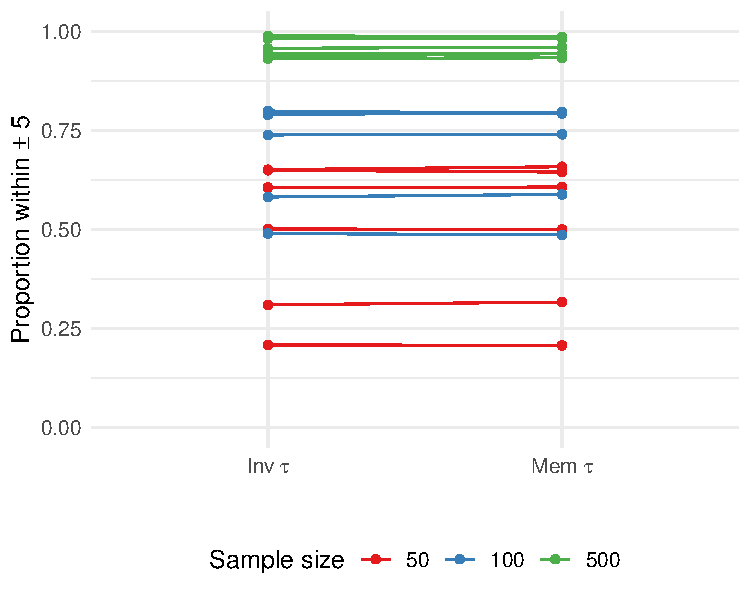
\includegraphics[width=\textwidth]{exp1_plplot.pdf}
         \caption{One change-point.}
         \label{fig:exp1plplot}
     \end{subfigure}
     \hfill
    \begin{subfigure}[b]{0.45\textwidth}
         \centering
         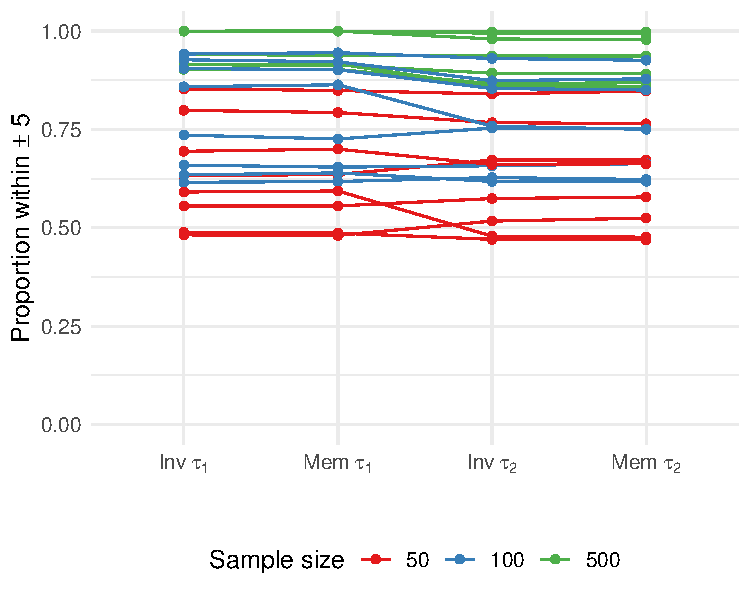
\includegraphics[width=\textwidth]{exp2_plplot.pdf}
         \caption{Two change-points.}
         \label{fig:exp2plplot}
     \end{subfigure}
     \begin{subfigure}[b]{0.45\textwidth}
         \centering
         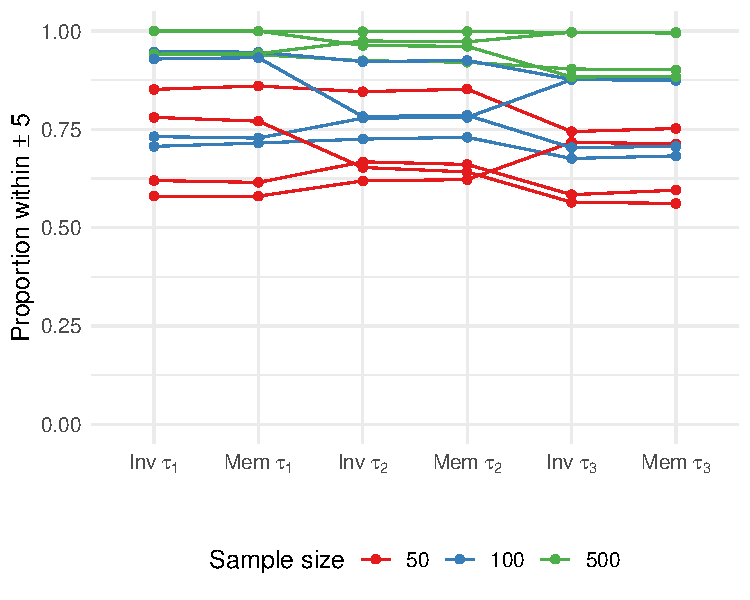
\includegraphics[width=\textwidth]{exp3_plplot.pdf}
         \caption{Three change-points.}
         \label{fig:exp3plplot}
     \end{subfigure}
     \hfill
     \begin{subfigure}[b]{0.45\textwidth}
         \centering
         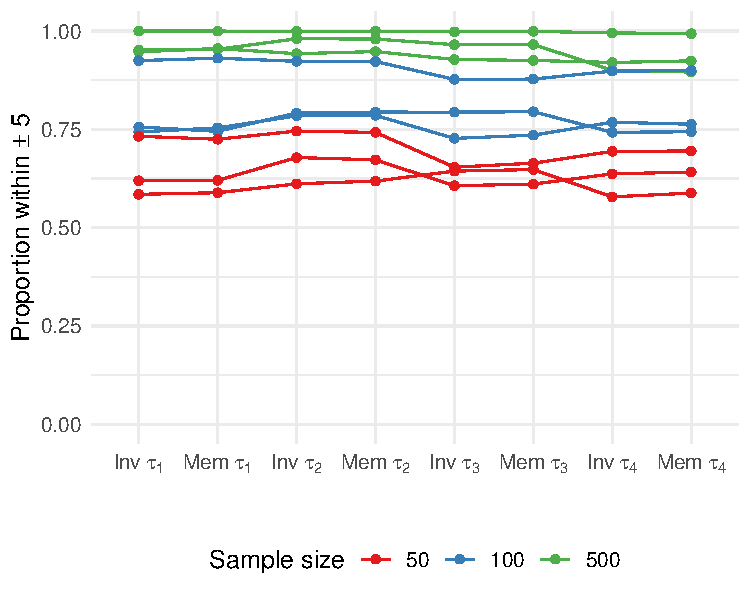
\includegraphics[width=\textwidth]{exp4_plplot.pdf}
         \caption{Four change-points.}
         \label{fig:exp4plplot}
     \end{subfigure}
    \caption{Accuracy of change-point simulations for the exponential distribution. The y-axis represents the proportion of change-point estimates ($\hat{\tau}$) within 10\% of the known value. ``Inv'' refers to the inverse hazard method and ``Mem'' refers to the memoryless method. This figure demonstrates that accuracy is higher with a larger sample size and is similar for both simulation methods.}
    \label{fig:expplplots}
\end{figure}


Simulations for the Weibull distribution, however, revealed important differences in accuracy between the two methods (see Figure~\ref{fig:weibplplots}). Although accuracy of the two methods was similar when simulating one change-point, there were many cases where accuracy was very low, even with a sample size of 500 (Figure~\ref{fig:weib1plplot}). In almost one quarter ($4/18$) of the simulation scenarios, the true value of $\tau$ was not within the 95\% confidence interval of the average estimate for either method. In three of those scenarios, both simulation methods severely underestimated $\tau$ when the true value was 80. When simulating two change-points (Figure~\ref{fig:weib2plplot}), accuracy of the first change-point was often much lower when using the memoryless method, especially with a larger sample size. All except one of the simulation scenarios where the known value of $\tau_1$ did not fall within the 95\% confidence interval of the average estimate for the memoryless method had a sample size of 500. Accuracy was lower for all change-points in the three change-point simulations when using the memoryless method and the discrepancies between the two methods were larger for larger sample sizes (Figure~\ref{fig:weib3plplot}). In almost half of the simulation scenarios at least one value of $\tau_i$ was not within the 95\% confidence interval of the mean estimate for the memoryless method and all except one of those scenarios had a sample size of 500. When simulating four change-points (Figure~\ref{fig:weib4plplot}), for most scenarios there was a large drop in accuracy at the first and third change-point for the memoryless method compared to the inverse hazard method. At the second and fourth change-points, however, there was a drop in accuracy for sample sizes of 50 and 100 whereas most simulation scenarios with a sample size of 500 had similar accuracy between the two methods. Every simulation scenario for four change-points with a sample size of 500 using the memoryless method had at least one change-point where the 95\% confidence interval did not include the known value of $\tau_i$. The known value of $\tau_4$ was, however, included in the 95\% confidence interval for every scenario with a sample size of 500.

\begin{figure}[ht]
    \centering
     \begin{subfigure}[b]{0.45\textwidth}
         \centering
         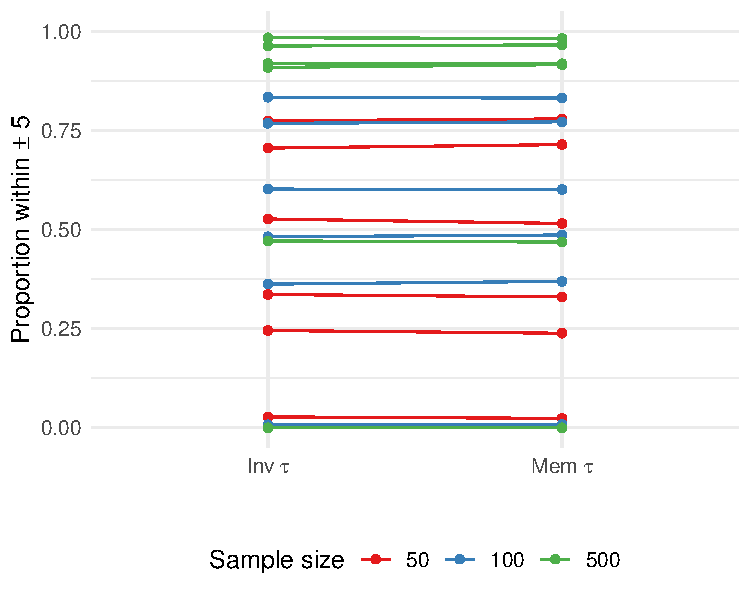
\includegraphics[width=\textwidth]{weib1_plplot.pdf}
         \caption{One change-point.}
         \label{fig:weib1plplot}
     \end{subfigure}
     \hfill
    \begin{subfigure}[b]{0.45\textwidth}
         \centering
         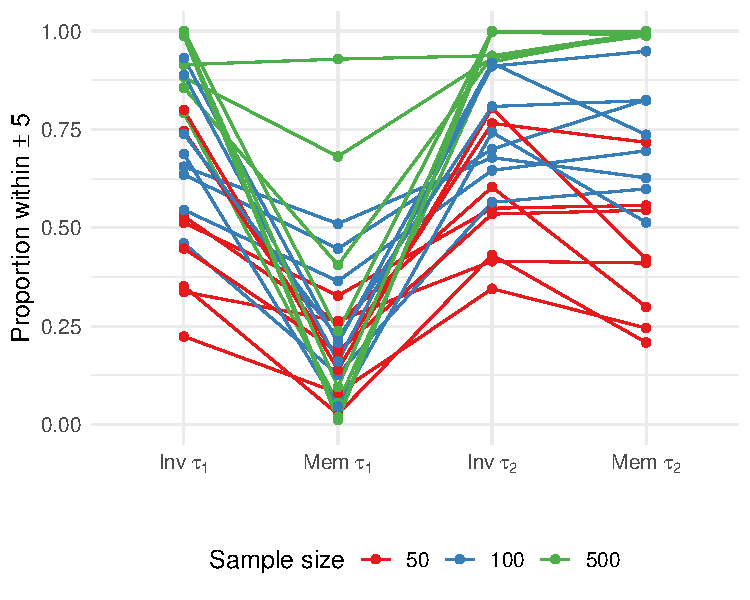
\includegraphics[width=\textwidth]{weib2_plplot.pdf}
         \caption{Two change-points.}
         \label{fig:weib2plplot}
     \end{subfigure}
     \\
     \begin{subfigure}[b]{0.45\textwidth}
         \centering
         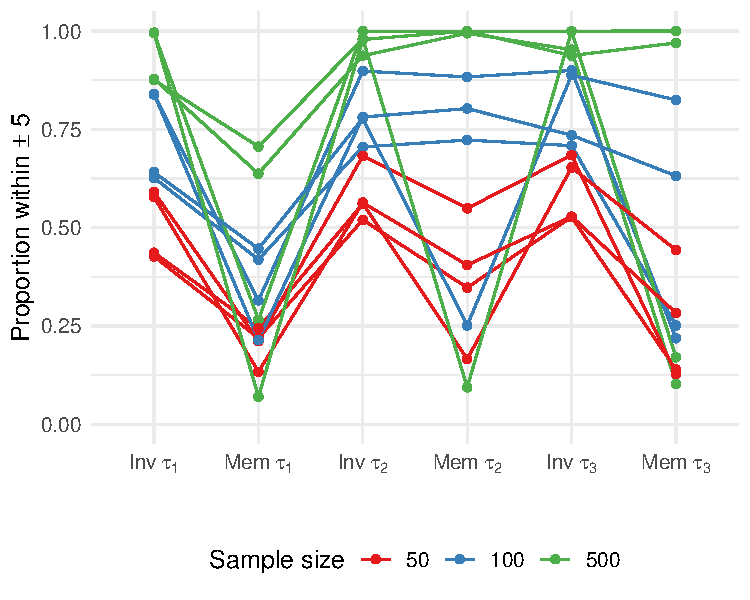
\includegraphics[width=\textwidth]{weib3_plplot.pdf}
         \caption{Three change-points.}
         \label{fig:weib3plplot}
     \end{subfigure}
     \hfill
     \begin{subfigure}[b]{0.45\textwidth}
         \centering
         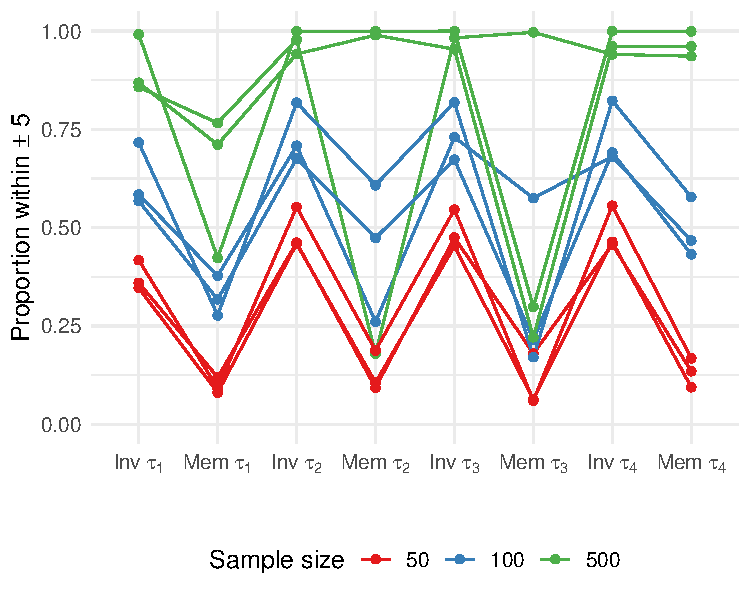
\includegraphics[width=\textwidth]{weib4_plplot.pdf}
         \caption{Four change-points.}
         \label{fig:weib4plplot}
     \end{subfigure}
    \caption{Accuracy of change-point simulations for the Weibull distribution. The y-axis represents the proportion of change-point estimates ($\hat{\tau}$) within 10\% of the known value. ``Inv'' refers to the inverse hazard method and ``Mem'' refers to the memoryless method. This figure demonstrates that accuracy is generally higher with larger sample sizes and when using the inverse hazard method.}
    \label{fig:weibplplots}
\end{figure}

We suspected that the inaccurate estimates using the Weibull distribution were due to inaccuracies in estimating the shape parameter $\gamma$, which is assumed constant across all time intervals. Indeed, $\gamma$ was often under-estimated as seen in Figure~\ref{fig:weibgplots}. Values of $\gamma$, however, were similar for both methods except when there were three change-points (Figure~\ref{fig:weib3gplot}), in which case the estimates of $\gamma$ using the inverse hazard method were closer to the known value of two. We were unable to estimate $\gamma$ for the simulations using the memoryless method when there was a sample size of 50 (Figure~\ref{fig:weib4gplot}). 

\begin{figure}[ht]
    \centering
     \begin{subfigure}[b]{0.45\textwidth}
         \centering
         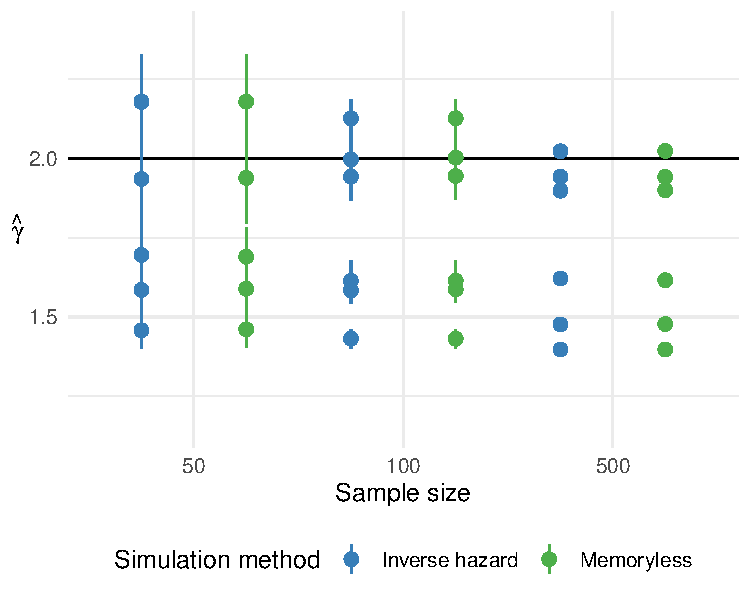
\includegraphics[width=\textwidth]{weib1_gplot.pdf}
         \caption{One change-point.}
         \label{fig:weib1gplot}
     \end{subfigure}
     \hfill
    \begin{subfigure}[b]{0.45\textwidth}
         \centering
         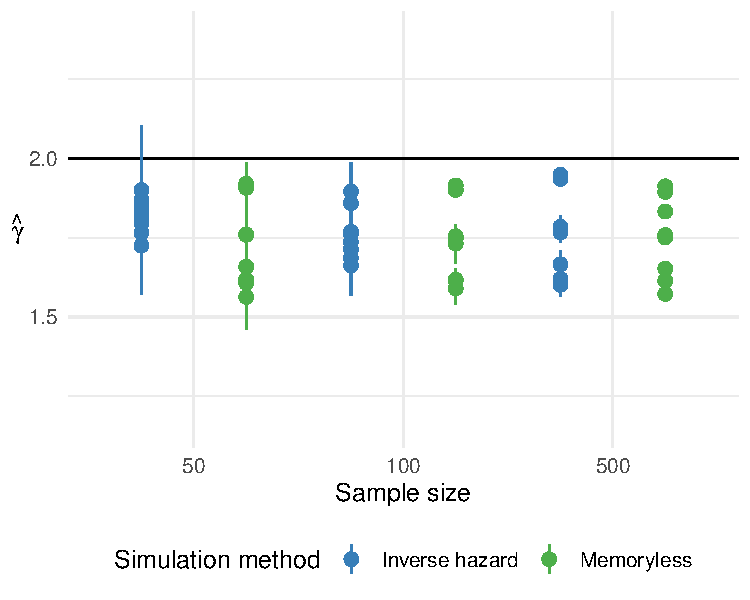
\includegraphics[width=\textwidth]{weib2_gplot.pdf}
         \caption{Two change-points.}
         \label{fig:weib2gplot}
     \end{subfigure}
     \\
     \begin{subfigure}[b]{0.45\textwidth}
         \centering
         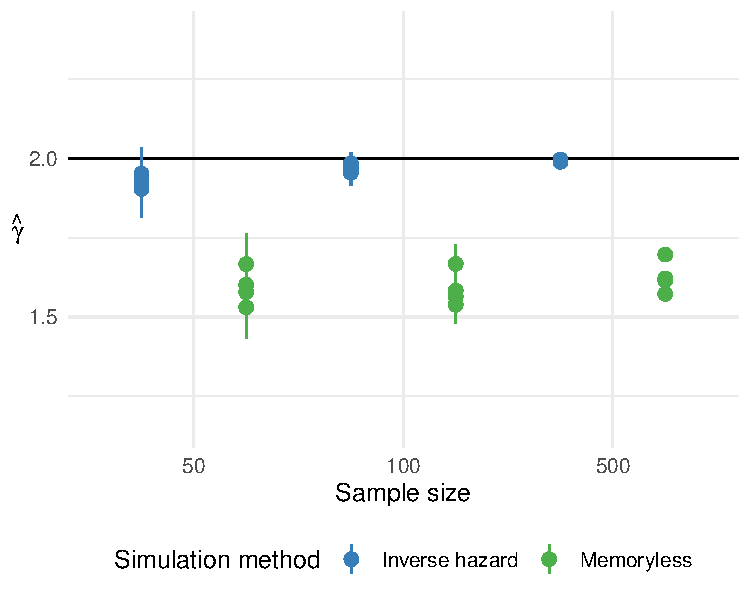
\includegraphics[width=\textwidth]{weib3_gplot.pdf}
         \caption{Three change-points.}
         \label{fig:weib3gplot}
     \end{subfigure}
     \hfill
     \begin{subfigure}[b]{0.45\textwidth}
         \centering
         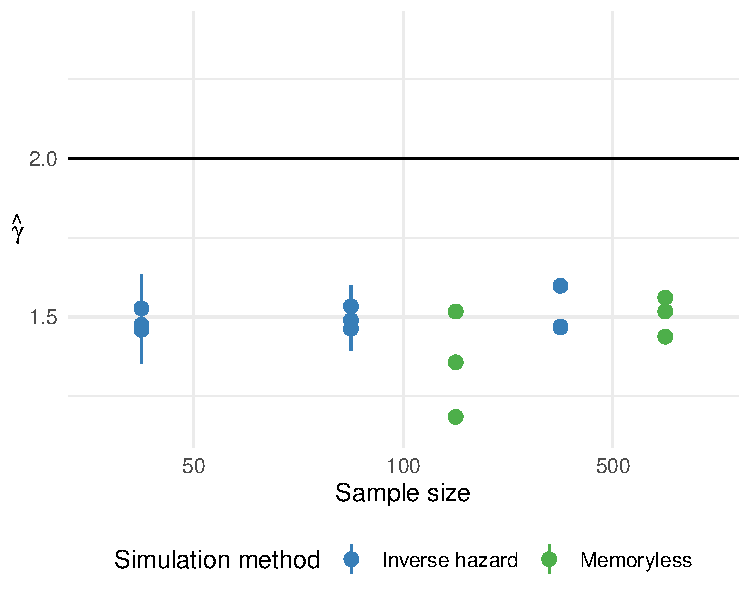
\includegraphics[width=\textwidth]{weib4_gplot.pdf}
         \caption{Four change-points.}
         \label{fig:weib4gplot}
     \end{subfigure}
    \caption{Estimated values of shape parameter $\gamma$ for the Weibull distribution. Dots indicate the average estimated value for each simulation scenario with the vertical lines representing the 95\% CI. The solid horizontal line represents the known value of $\gamma$. This plot demonstrates inaccurate estimates of $\gamma$ for both simulation methods except when there are three change-points, in which case the estimates are more accurate using the inverse hazard method.}
    \label{fig:weibgplots}
\end{figure}

\section{Summary}

The R package \pkg{cpsurvsim} provides implementation of the standard method of simulating from a distribution, using the inverse CDF, and a new method that exploits the memoryless property of survival analysis. When simulating from the exponential distribution with multiple change-points, these methods have comparable performance. Simulating multiple change-points from the Weibull hazard, however, suggested that the inverse hazard method produces more accurate estimates of the change-points $\tau_i$. The accuracy of the exponential simulations suffered when the sample size was less than 500 whereas in some cases, simulations of the Weibull distribution had worse accuracy with a sample size of 500. In practice, change-point hazard models are often applied to data from large longitudinal cohort studies where the sample size is very large (e.g., \cite{Goodman} and \cite{Williams}). These results suggest that larger sample sizes are preferred when using an exponential model but to use caution even with a large sample when using the Weibull model. We hope that having an R package for simulating data from multiple change-point hazard distributions will aid in the development of extensions and alternatives to our research on tests for multiple change-points \citep{Hochheimer2}. 

The inspiration to develop the memoryless simulation method and test it came from observing the shortcomings of the inverse hazard method in our research. The memoryless method performs better in some simulation scenarios, which led us to implement both methods in this R package. This simulation study, however, suggests that in the majority of cases the inverse hazard method simulates values of $\tau_i$ more accurately. Our simulation study also highlighted accuracy issues with both methods when simulating data from sample sizes of 50 or 100, which we suspect are due to using a relatively small amount of data to estimate several model parameters. One should consider exploring other methods to simulate a multiple change-point distribution with a small sample size. The acceptance-rejection method, for example, may produce more accurate parameter estimates at the cost of more computational time needed to reach the desired sample size, a cost that might be worthwhile if the sample size is smaller to begin with \citep{StatComp}. Alternatively, one might run a simulation study to determine which of these two methods is best suited for their specific parameters.

An important limitation of the \code{exp\_cdfsim} and \code{weib\_cdfsim} functions is that they only accommodate up to four change-points. While it's possible to have more than this many change-points in a dataset, it's also important to make sure that there is a meaningful interpretation for multiple change-points. Also, \pkg{cpsurvsim} only accommodates type I right censoring. For the Weibull distribution, $\gamma$ is assumed fixed for every interval between change-points. In our simulation study, we only estimated an overall value of $\gamma$ due to convergence issues when trying to estimate it within each interval between change-points. In an effort to be concise, the accuracy of the scale parameters $\theta_i$ are not discussed here, however, in some cases this parameter may be of more interest than the change-point $\tau$. Thus, we briefly discuss these results in the appendix. Future versions of \pkg{cpsurvsim} could incorporate additional features such as accommodating informative censoring. 

\section{Acknowledgments}
Thank you to Dr. Sarah Ratcliffe for her guidance and for assisting with running these simulations.

\bibliography{Hochheimer-Sabo}


\address{Camille J. Hochheimer, PhD\\
  Department of Biostatistics and Informatics\\
  Colorado School of Public Health\\
  13001 East 17th Place, 4th Floor West, Aurora, CO 80045\\
  USA\\
  ORCiD: 0000-0002-0984-0909\\
  \email{camille.hochheimer@cuanschutz.edu}}

\address{Roy T. Sabo, PhD\\
  Department of Biostatistics \\
  Virginia Commonwealth University\\
  PO Box 980032, Richmond, VA 23298-0032\\
  USA\\
  ORCiD: 0000-0001-9159-4876\\
  \email{roy.sabo@vcuhealth.org}}

\newpage

\begin{appendix}

\section{Appendix: Analysis of scale parameters}

While the change-points can be estimated without knowing the values of the scale parameters, the reverse is not possible. Thus, we used the estimated values of the change-points in order to estimate values of $\theta_i$. As the number of change-points increased, so did the difficulty in estimating values of $\theta_i$, especially with a smaller sample size. 

With a few exceptions, the estimates of $\theta_i$ for the exponential distribution were similar between both methods (Figure~\ref{fig:exptplots}). These exceptions were $\theta_2$ in the two change-point (Figure~\ref{fig:exp2tplot}) and three change-point models (Figure~\ref{fig:exp3tplot}), where the memoryless method with a sample size of 100 had a much larger proportion of bias. We were only able to estimate the shape parameters for the four change-point model when the sample size was 500.

\begin{figure}[ht]
    \centering
     \begin{subfigure}[b]{0.45\textwidth}
         \centering
         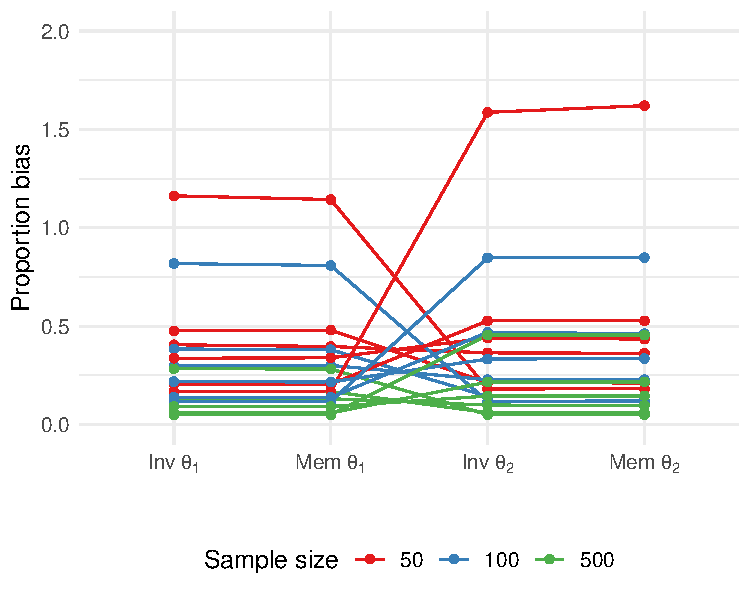
\includegraphics[width=\textwidth]{exp1_tplot.pdf}
         \caption{One change-point.}
         \label{fig:exp1tplot}
     \end{subfigure}
     \hfill
    \begin{subfigure}[b]{0.45\textwidth}
         \centering
         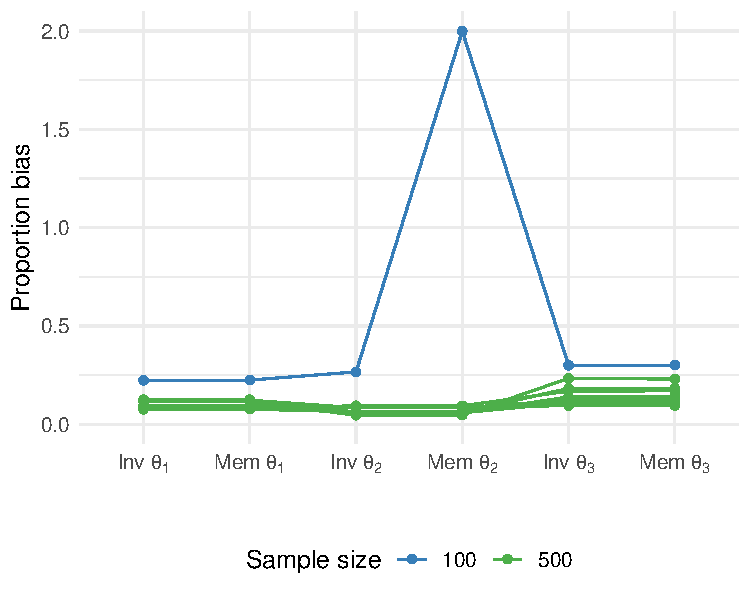
\includegraphics[width=\textwidth]{exp2_tplot.pdf}
         \caption{Two change-points.}
         \label{fig:exp2tplot}
     \end{subfigure}
     \begin{subfigure}[b]{0.45\textwidth}
         \centering
         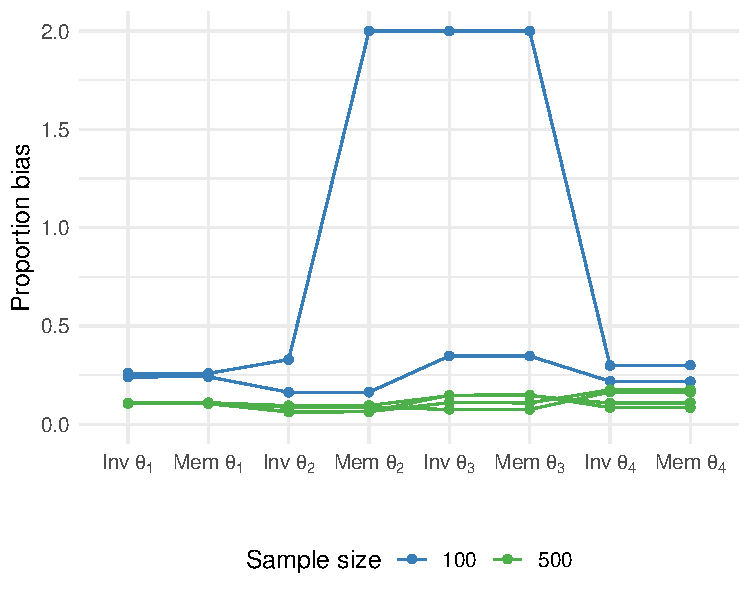
\includegraphics[width=\textwidth]{exp3_tplot.pdf}
         \caption{Three change-points.}
         \label{fig:exp3tplot}
     \end{subfigure}
     \hfill
     \begin{subfigure}[b]{0.45\textwidth}
         \centering
         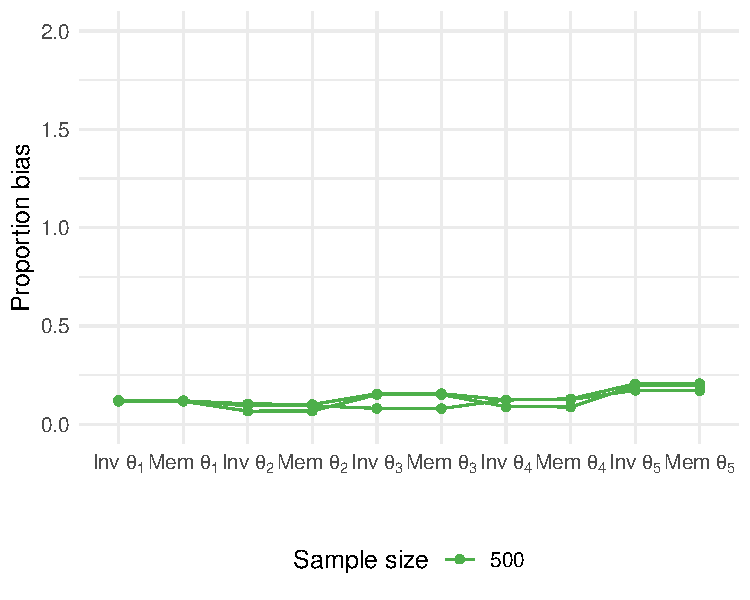
\includegraphics[width=\textwidth]{exp4_tplot.pdf}
         \caption{Four change-points.}
         \label{fig:exp4tplot}
     \end{subfigure}
    \caption{Accuracy of scale parameter $\hat{\theta_i}$ for the exponential distribution. The y-axis represents the average proportion of bias of $\hat{\theta_i}$ relative to the known value of $\theta_i$. A proportion of bias of 2 represents estimates with at least 200\% bias. ``Inv'' refers to the inverse hazard method and ``Mem'' refers to the memoryless method. This figure demonstrates that bias was generally similar between simulation methods with a few exceptions where bias was larger using the memoryless method.}
    \label{fig:exptplots}
\end{figure}

Estimates of $\theta_i$ for the one change-point Weibull model were similar across simulation methods but bias was high even when the sample size was large (Figure~\ref{fig:weib1tplot}). Bias was generally smaller when using the memoryless method to estimate $\theta_i$ in the two change-point Weibull model (Figure~\ref{fig:weib2tplot}). On the other hand, bias was larger when using the memoryless method to estimate the shape parameter for the three change-point Weibull model (Figure~\ref{fig:weib3tplot}). We were unable to estimate $\theta$ using the results from the memoryless method for any of the four change-point simulations.

\begin{figure}[ht]
    \centering
     \begin{subfigure}[b]{0.45\textwidth}
         \centering
         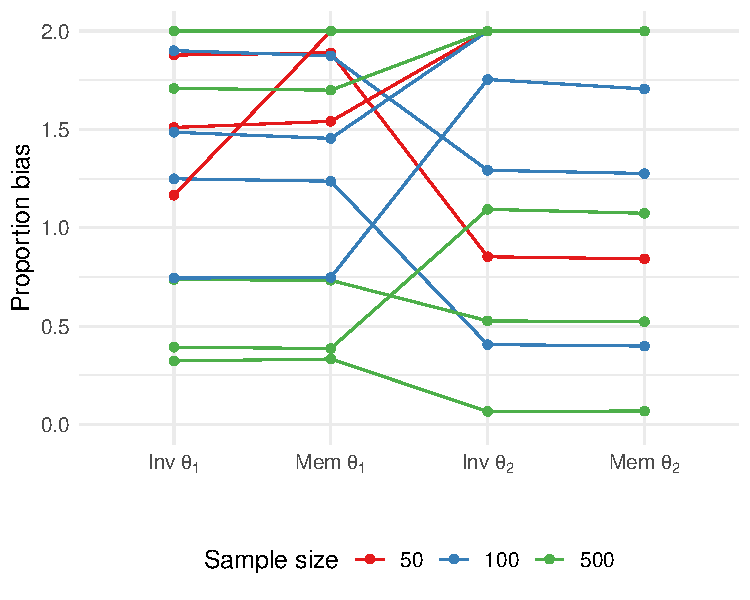
\includegraphics[width=\textwidth]{weib1_tplot.pdf}
         \caption{One change-point.}
         \label{fig:weib1tplot}
     \end{subfigure}
     \hfill
    \begin{subfigure}[b]{0.45\textwidth}
         \centering
         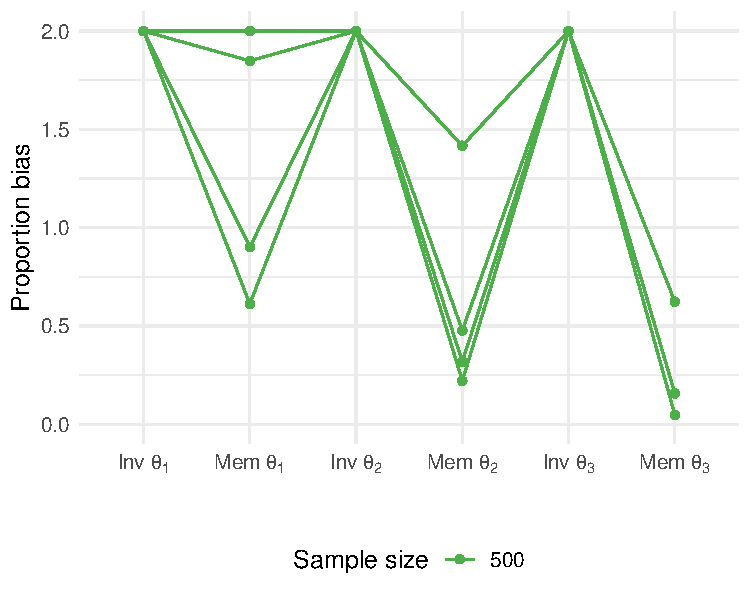
\includegraphics[width=\textwidth]{weib2_tplot.pdf}
         \caption{Two change-points.}
         \label{fig:weib2tplot}
     \end{subfigure}
     \begin{subfigure}[b]{0.70\textwidth}
         \centering
         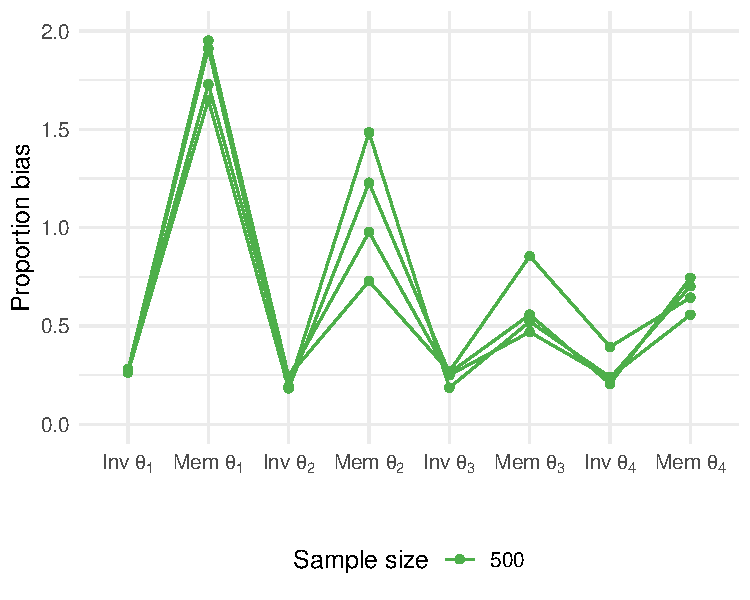
\includegraphics[width=\textwidth]{weib3_tplot.pdf}
         \caption{Three change-points.}
         \label{fig:weib3tplot}
     \end{subfigure}
    \caption{Accuracy of scale parameter $\hat{\theta_i}$ for the Weibull distribution. The y-axis represents the average proportion of bias of $\hat{\theta_i}$ relative to the known value of $\theta_i$. A proportion of bias of 2 represents estimates with at least 200\% bias. ``Inv'' refers to the inverse hazard method and ``Mem'' refers to the memoryless method. This figure demonstrates similar bias between methods when there is one change-point, smaller bias using the memoryless method when there are two change-points, and smaller bias using the inverse hazard method when there are three change-points.}
    \label{fig:weibtplots}
\end{figure}

\end{appendix}